%%%%%%%%%%%%%%%%%%%%%%%%%%%%%%%%%%%%%%%%%%%%%%%%%%%%%%%%%%%%%%%%%%%%%%%%%%%%%%%%
% test.tex
%%%%%%%%%%%%%%%%%%%%%%%%%%%%%%%%%%%%%%%%%%%%%%%%%%%%%%%%%%%%%%%%%%%%%%%%%%%%%%%%
%
% Authors:
% - Sébastien Julliot
%
% Contributors:
% - Unknown for now
%
%%%%%%%%%%%%%%%%%%%%%%%%%%%%%%%%%%%%%%%%%%%%%%%%%%%%%%%%%%%%%%%%%%%%%%%%%%%%%%%%


\documentclass{42}

\usepackage{amsmath, amsfonts, amssymb}


%%%%%%%%%%%%%%%%%%%%%%%%%%%%%%%%%%%%%%%%%%%%%%%%%%%%%%%%%%%%%%%%%%%%%%%%%%%%%%%%
% Prologue
%%%%%%%%%%%%%%%%%%%%%%%%%%%%%%%%%%%%%%%%%%%%%%%%%%%%%%%%%%%%%%%%%%%%%%%%%%%%%%%%

\begin{document}

%Table des matieres
\title{Computor v1}
\subtitle{}

\member {42 staff}{staff@42.fr}

\summary
{

	Ce projet est le premier d'une série ayant pour but de vous faire renouer avec les maths, qui vous seront très utiles -voire nécessaires- pour de nombreux autres projets.
}

\maketitle

\tableofcontents

% Valeurs utilisees pour la generation de headers d'exercices
\turnindir{svn+ssh://rendus@rendus.42.fr/sujetdetest-2142-login\_x}


\graphicspath{{images/}}

\newpage
%%%%%%%%%%%%%%%%%%%%%%%%%%%%%%%%%%%%%%%%%%%%%%%%%%%%%%%%%%%%%%%%%%%%%%%%%%%%%%%%
% Start document
%%%%%%%%%%%%%%%%%%%%%%%%%%%%%%%%%%%%%%%%%%%%%%%%%%%%%%%%%%%%%%%%%%%%%%%%%%%%%%%%

\chapter{Préambule}
\begin{flushleft}
Un polynôme est une expression formelle de la forme:
	\begin{equation}
	P(X)=\sum_{k=0}^{n} a_k X^k
	\end{equation}
	où X est appelé indéterminée du polynôme.
	\newline
	\newline
	Le produit de deux polynômes est ainsi défini par
	\begin{equation}
	\left(\sum_{i=0}^n a_iX^i\right)\left(\sum_{j=0}^m b_jX^j\right) = \sum_{k=0}^{n+m} \left(\sum_{i+j = k}a_ib_j\right)X^k.
	\end{equation}
\end{flushleft}
\begin{center}
	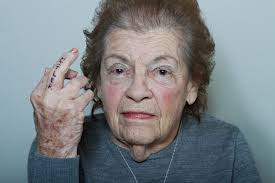
\includegraphics[scale=0.35]{what1}
	
\includegraphics[scale=0.35]{what2}
	
\includegraphics[scale=0.35]{what3}
	
\includegraphics[scale=0.35]{what4}
	
\includegraphics[scale=0.35]{what5}
	
\includegraphics[scale=0.35]{what6}
	
\includegraphics[scale=0.35]{what7}
	
\includegraphics[scale=0.35]{what8}
\end{center}

\hint
{
	La video offre une explication plus ... comprehensible.
}

\newpage

\chapter{Introduction}

Le but de ce sujet est de vous faire coder un programme qui résout des équations simples.

Ainsi le programme prendra en paramètre une équation (polynomiale, c'est-à-dire ne faisant intervenir que des puissances, aucune fonction compliquée) et affichera sa (ses) solution(s).

Pourquoi des polynômes? Parce que c'est l'un des outils mathématiques les plus simples et les plus puissants. On s'en sert dans tous les domaines et à tous les niveaux pour $simplifier$ et $exprimer$ beaucoup de choses. Les fonctions $sin$, $cos$, et $tan$ par exemple sont calculées à l'aide de polynômes.

\info
{
En fait, il existe même un résultat ,le théorème de Stone-Weierstrass, qui dit que toutes les fonctions "courantes", (celles qui sont bien lisses et jolies), peuvent être exprimées à l'aide de polynômes.
}

\chapter{Objectifs}

L’idée est de vous faire reprendre contact avec la manipulation d'outils mathématiques élémentaires, qui pourront vous être utiles dans de nombreux autres sujets de 42. Il ne s'agit donc pas de "faire des maths pour faire des maths" mais de vous permettre d'aborder plus progressivement et sereinement les sujets faisant intervenir des maths (notamment le mod1 pour ce sujet).

Voici une liste non exhaustive des sujets où savoir ce que sont et comment manipuler les polynômes pourrait bien vous être utile:
	\begin{itemize}
	\item Fractol
	\item RT
	\item mod1
	\item Expert System
	\item Infin Mult
\end{itemize}

Par ailleurs, ce petit sujet sera complété par d'autres sur des sujets variés, pour comprendre ce que vous faites plutôt que simplement copier une formule sur Internet.

\chapter{Partie obligatoire}

\extitle{Computor v1}
\exfiles{A votre convenance}

\makeheaderbasic

Le but de l'exercice est d'écrire un programme qui résout des équations polynomiales.

Exemples:

\begin{42console}
Entrez une equation: 5 * X^0 + 4 * X^1 - 9.3 * X^2 = 1 * X^0
Sous forme reduite : 4 * X^0 + 4 * X^1 - 9.3 * X^2 = 0
Cette equation est de degre 2.
Son discriminant est strictement positif, elle a donc exactement deux solutions reelles :
0.905239
-0.475131
\end{42console}

\begin{42console}
Entrez une equation: 5 * X^0 + 4 * X^1 = 4 * X^0
Sous forme reduite : 1 * X^0 + 4 * X^1 = 0
Cette equation est de degre 1 et a pour solution -0.25.
\end{42console}

\begin{42console}
Entrez une equation: 8 * X^0 - 6 * X^1 + 0 * X^2 - 5.6 * X^3 = 3 * X^0
Sous forme reduite : 5 * X^0 - 6 * X^1 + 0 * X^2 - 5.6 * X^3 = 0
L'equation est de degre superieur a 2, on ne sait pas resoudre.
\end{42console}

NB: Pour la partie obligatoire, on considèrera l'entrée bien formatée (ie. tous les termes sont de la forme \begin{equation}coefficient * X^{puissance}\end{equation}. Les puissances sont bien ordonnées et toutes présentes.

\info
{
	La résolution des équations de degré trois ou plus n'est pas demandée, et sera envisagée ultérieurement.
}

\newpage

\chapter{Partie bonus}

Voici une liste de bonus qu'il pourrait être utile d'implémenter:



\begin{itemize}
	\item Gérer les erreurs sur l'entrée
	\item Gérer les entrées sorties sous forme naturelle
\begin{42console}
Entrez une equation: 5 + 4 * X + X^2= X^2
Sous forme reduite : 5 + 4 * X = 0
Cette equation est de degre 1 et a pour solution -1.25.
\end{42console}
	\item Afficher la (les) solution sous forme de fraction irréductible quand c'est intéressant
	\item Afficher des étapes intermédiaires
	\item ...
\end{itemize}

\chapter{Consignes}
\begin{flushleft}
	\begin{itemize}
		\item Pensez aux solutions complexes quand le degré vaut 2 ;)
		\item Le choix du langage est à votre discrétion.

		\item Cela dit, vous n'avez évidemment droit à aucune fonction mathématique (hors addition et multiplication de réels) que vous n'ayez pas implémentée vous-mêmes.

		\item Si vous travaillez dans un langage compilable (C/C++ notamment), vous rendrez un Makefile contenant les règles habituelles.
		\item En C, vous respecterez bien sûr la norme.
	\end{itemize}
\end{flushleft}
Bon courage !

%%%%%%%%%%%%%%%%%%%%%%%%%%%%%%%%%%%%%%%%%%%%%%%%%%%%%%%%%%%%%%%%%%%%%%%%%%%%%%%%
% End document
%%%%%%%%%%%%%%%%%%%%%%%%%%%%%%%%%%%%%%%%%%%%%%%%%%%%%%%%%%%%%%%%%%%%%%%%%%%%%%%%
\end{document}
